\documentclass[12pt,a4paper,]{article}
\usepackage[]{mathpazo}
\usepackage{setspace}
\setstretch{2}
\usepackage{amssymb,amsmath}
\usepackage{ifxetex,ifluatex}
\usepackage{fixltx2e} % provides \textsubscript
\ifnum 0\ifxetex 1\fi\ifluatex 1\fi=0 % if pdftex
  \usepackage[T1]{fontenc}
  \usepackage[utf8]{inputenc}
\else % if luatex or xelatex
  \ifxetex
    \usepackage{mathspec}
  \else
    \usepackage{fontspec}
  \fi
  \defaultfontfeatures{Ligatures=TeX,Scale=MatchLowercase}
\fi
% use upquote if available, for straight quotes in verbatim environments
\IfFileExists{upquote.sty}{\usepackage{upquote}}{}
% use microtype if available
\IfFileExists{microtype.sty}{%
\usepackage[]{microtype}
\UseMicrotypeSet[protrusion]{basicmath} % disable protrusion for tt fonts
}{}
\PassOptionsToPackage{hyphens}{url} % url is loaded by hyperref
\usepackage[unicode=true]{hyperref}
\PassOptionsToPackage{usenames,dvipsnames}{color} % color is loaded by hyperref
\hypersetup{
            pdftitle={ Trade-offs among plant floral and reproductive traits determine interactions with floral visitors},
            colorlinks=true,
            linkcolor=RoyalBlue,
            citecolor=Blue,
            urlcolor=RoyalBlue,
            breaklinks=true}
\urlstyle{same}  % don't use monospace font for urls
\usepackage[margin=1in]{geometry}
\usepackage{longtable,booktabs}
% Fix footnotes in tables (requires footnote package)
\IfFileExists{footnote.sty}{\usepackage{footnote}\makesavenoteenv{long table}}{}
\usepackage{graphicx,grffile}
\makeatletter
\def\maxwidth{\ifdim\Gin@nat@width>\linewidth\linewidth\else\Gin@nat@width\fi}
\def\maxheight{\ifdim\Gin@nat@height>\textheight\textheight\else\Gin@nat@height\fi}
\makeatother
% Scale images if necessary, so that they will not overflow the page
% margins by default, and it is still possible to overwrite the defaults
% using explicit options in \includegraphics[width, height, ...]{}
\setkeys{Gin}{width=\maxwidth,height=\maxheight,keepaspectratio}
\IfFileExists{parskip.sty}{%
\usepackage{parskip}
}{% else
\setlength{\parindent}{0pt}
\setlength{\parskip}{6pt plus 2pt minus 1pt}
}
\setlength{\emergencystretch}{3em}  % prevent overfull lines
\providecommand{\tightlist}{%
  \setlength{\itemsep}{0pt}\setlength{\parskip}{0pt}}
\setcounter{secnumdepth}{0}

% set default figure placement to htbp
\makeatletter
\def\fps@figure{htbp}
\makeatother

\usepackage{lineno} % add 
\linenumbers % turns line numbering on 

% Allowing for landscape pages
\usepackage{lscape}
\newcommand{\blandscape}{\begin{landscape}}
\newcommand{\elandscape}{\end{landscape}}

% Left justification of the text: see https://www.sharelatex.com/learn/Text_alignment
% \usepackage[document]{ragged2e} % already in the latex template
\newcommand{\bleft}{\begin{flushleft}}
\newcommand{\eleft}{\end{flushleft}}


% Add Supplementary Tables and Figures
% Code from https://stackoverflow.com/a/51337664
\newcommand{\beginsupplement}{
  \setcounter{table}{0}  
  \renewcommand{\thetable}{S\arabic{table}}
  \setcounter{figure}{0} 
  \renewcommand{\thefigure}{S\arabic{figure}}
}
\usepackage{booktabs}
\usepackage{longtable}
\usepackage{array}
\usepackage{multirow}
\usepackage{wrapfig}
\usepackage{float}
\usepackage{colortbl}
\usepackage{pdflscape}
\usepackage{tabu}
\usepackage{threeparttable}
\usepackage{threeparttablex}
\usepackage[normalem]{ulem}
\usepackage{makecell}
\usepackage{xcolor}
\usepackage{float}
\floatplacement{figure}{H}
\usepackage[skip=3pt]{caption}
\captionsetup[figure]{labelformat=empty}
\usepackage{setspace}
\usepackage{titlesec}
\titlespacing{\title}{0pt}{\parskip}{-\parskip}
\usepackage[style=nature]{biblatex}
\usepackage[labelformat = empty]{caption}
\usepackage{float}
\usepackage{booktabs}
\usepackage{longtable}
\usepackage{array}
\usepackage{multirow}
\usepackage{wrapfig}
\usepackage{colortbl}
\usepackage{pdflscape}
\usepackage{tabu}
\usepackage{threeparttable}
\usepackage{threeparttablex}
\usepackage[normalem]{ulem}
\usepackage{makecell}
\usepackage{xcolor}

\title{\singlespacing \vspace{-1.5cm} \LARGE Trade-offs among plant floral and
reproductive traits determine interactions with floral visitors}
\author{}
\date{\vspace{-2.5em}}

\begin{document}
\maketitle

\vspace{-2.2cm} \singlespacing
\large 
\textbf{Jose B. Lanuza$^{1,2}*$, Romina Rader$^{1}$, Jamie Stavert$^{3}$, Liam K. Kendall$^{4}$, Manu E. Saunders$^{1}$ and Ignasi Bartomeus$^{2}$}

\normalsize

\textbf{Plant life strategies are often delimited by vegetative and
physiological traits but little is known about how floral and
reproductive traits drive these strategies, and in turn shape plant
interactions with floral visitors. Here, we compiled 13 floral, 4
reproductive and 3 vegetative traits for 1,506 plant species from 28
plant-pollinator network studies across 18 different countries. We
investigated the associations among these traits, pollinator visitation
and the functional role of plant species within the networks
(interaction frequency, normalized degree and specialization). We found
that 51.8\% of trait variation was explained by two independent axes
that encompassed plant form and function. Specifically, the first axis
indicated the presence of a trade-off between flower number and flower
size (PC1, 26.72\%). The second axis indicated a trade-off for the level
of pollinator dependency (PC2, 25.08\%). Although the main axes of trait
variation did not fully explain pollinator visitation rates, different
plant life strategies were associated with visitation rates and
pollinator functional groups. Overall, the main traits that determined
plant species' functional roles were height, nectar concentration,
pollen grains per flower, number of ovules, style length, selfing level
and flower width. Our results highlight the need to consider plant
reproductive and floral traits to improve understanding of plant life
strategies and plant-pollinator interactions at broader spatial scales.}

\small
\vspace{-0.5cm}

\noindent\rule{\textwidth}{1pt}

\textsuperscript{1} School of Environmental and Rural Science,
University of New England, Armidale, New South Wales 2350, Australia.
\textsuperscript{2} Estación Biológica de Doñana (EBD-CSIC), E-41092
Seville, Spain. \textsuperscript{3} Department of Conservation
\textbar{} Te Papa Atawhai, Auckland, New Zealand. \textsuperscript{4}
Centre for Environmental and Climate Science, Lund University,
Sölvegatan 37, S-223 62 Lund, Sweden. \texttt{*} e-mail:
\href{mailto:barragansljose@gmail.com}{\nolinkurl{barragansljose@gmail.com}}

\doublespacing
\vspace{5mm} \bleft
\normalsize

There is an astonishing diversity of floral structures and plant
reproductive strategies among flowering
plants\textsuperscript{\protect\hyperlink{ref-barrett2002}{1},\protect\hyperlink{ref-schiestl2013}{2}},
which have long been of interest to pollination biologists in terms of
their relevance to plant-pollinator interactions. However, most studies
that have explored reproductive (e.g., mating and compatibility systems)
and floral trait (e.g., flower size or nectar provision) variation have
concentrated on the individual or community level and thus, broader
macroecological patterns remain poorly
investigated\textsuperscript{\protect\hyperlink{ref-carvalheiro2014}{3}--\protect\hyperlink{ref-grossenbacher2017}{7}}.
Indeed, studies depicting species' life history strategies generally
focus on vegetative traits and rarely consider reproductive
traits\textsuperscript{\protect\hyperlink{ref-salguero2016}{8}}. As a
consequence, a unified framework that explores the compromises among
floral traits and their relevance to plant life strategies is currently
lacking\textsuperscript{\protect\hyperlink{ref-roddy2021}{10}}. At the
same time, there is growing interest in the determinants of
plant-pollinator interactions via trait-based
approaches\textsuperscript{\protect\hyperlink{ref-fenster2004}{11}} and
trait-matching
analyses\textsuperscript{\protect\hyperlink{ref-bartomeus2016}{12}}.
However, floral traits have been overlooked beyond highly specialised
plant-pollinator
systems\textsuperscript{\protect\hyperlink{ref-roddy2021}{10},\protect\hyperlink{ref-dellinger2020}{13}}
and the role of plant reproductive biology remains little explored in
plant-pollinator interactions (but see
references\textsuperscript{\protect\hyperlink{ref-tur2013}{14},\protect\hyperlink{ref-devaux2014}{15}}).

With the recent availability of large trait databases, plant ecological
strategies are increasingly being
examined\textsuperscript{\protect\hyperlink{ref-kattge2011}{16},\protect\hyperlink{ref-salguero2015}{17}},
and are facilitating the identification of global patterns and
constraints of plant form and
function\textsuperscript{\protect\hyperlink{ref-salguero2016}{8},\protect\hyperlink{ref-diaz2016}{18},\protect\hyperlink{ref-carmona2021}{19}}.
However, the main focus has been on vegetative traits such as
leaf\textsuperscript{\protect\hyperlink{ref-wright2004}{20}} or
wood\textsuperscript{\protect\hyperlink{ref-chave2009}{21}} trade-offs
with little or no attention given to reproductive and floral
traits\textsuperscript{\protect\hyperlink{ref-evojtko2020}{22}}, also
critical to plant form and function. For instance, short lived versus
perennial species tend to have low versus high levels of outcrossing,
respectively\textsuperscript{\protect\hyperlink{ref-moeller2017}{6},\protect\hyperlink{ref-barrett2003}{23}}.
Further, outcrossing levels are positively correlated with flower
size\textsuperscript{\protect\hyperlink{ref-goodwillie2010}{24}}. In
addition, the presence of costly rewards (e.g., pollen or nectar) and
showy flowers or floral displays can only be understood through
consideration of plant species' reliance upon animal pollination
(pollinator dependence) and their role in attracting
pollinators\textsuperscript{\protect\hyperlink{ref-ollerton2011}{25}}.
Hence, exploring plant life strategies with reproductive and floral
trade-offs, in conjunction with their pollinator dependence, is
necessary for a balanced understanding of plant economics.

Several studies have identified links between plant traits and
plant-pollinator network
properties\textsuperscript{\protect\hyperlink{ref-carvalheiro2014}{3},\protect\hyperlink{ref-lazaro2008}{26},\protect\hyperlink{ref-bartomeus2013}{27}}.
Moreover, plant traits can also define species' network roles (e.g.,
specialists vs generalists). For example, species that occupy trait
space extremes are more likely to exhibit higher specialization and be
more reliant on
trait-matching\textsuperscript{\protect\hyperlink{ref-junker2013}{28},\protect\hyperlink{ref-coux2016}{29}}.
This morphological matching between plant and floral visitors can
determine plant-pollinator interactions, and thus shape their
interaction network
structure\textsuperscript{\protect\hyperlink{ref-stang2009}{30},\protect\hyperlink{ref-ibanez2012}{31}}.
Despite the increasing knowledge of the relevance of traits on the
species network roles, little is known about how plant reproductive and
floral traits determine plant species' network roles at a
macroecological scale.

Here, we explore the potential trade-offs among plant floral and
reproductive traits and how these influence the structure of
plant-pollinator networks. First, we identify the major axes of floral
and reproductive trait variation and trade-offs that determine plant
form and function. Second, we investigate how plant species' position in
trait-space influences interaction strength with different guilds of
floral visitors. Finally, we investigate how the main axes of trait
variation and individual traits influence plant species roles within
networks using complementary interaction network metrics (i.e.,
interaction strength, normalized degree and specialization).

\section{RESULTS}\label{results}

\textbf{Plant strategies.} The phylogenetically informed principal
component analysis (pPCA) captured by the first two and three axes
51.8\% and 70.97\% of trait variation, respectively (Fig. 1 and
Supplementary Fig. S5) and had a phylogenetic correlation (\(\lambda\))
of 0.76. The first principal component (PC1) represented 26.72\% of the
trait variation and indicated a trade-off between flower number and
flower size. We refer to this axis as the `flower number - flower size
trade-off' as already described in previous
studies\textsuperscript{\protect\hyperlink{ref-sargent2007}{32},\protect\hyperlink{ref-kettle2011}{33}}.
Hence, one end of the spectrum comprised species with high investment in
flower number and plant height but small flower size, short style length
and low ovule number. The other end of this spectrum comprised species
that were short in height and invested in large flowers, long styles,
many ovules, but few flowers. The main contributing traits to PC1 were
plant height, flower number, ovule number and flower size (loadings
\textgreater{} \textbar{}0.5\textbar{}; Supplementary Table S3) but
style length also contributed moderately on PC1 (loading = -0.33). The
second principal component (PC2) represented 25.05\% of the trait
variation and indicated a trade-off between low and high pollinator
dependence. We refer to this axis as the `pollinator dependence
trade-off'. The main driver of trait variation on PC2 was autonomous
selfing (loading = 0.85) but the other traits (except ovule number) also
made moderate contributions (loadings from 0.27 to 0.4; Supplementary
Table S3). We found that high pollinator dependence was associated with
larger and a higher number of flowers, greater plant height and longer
styles. In contrast, species with high levels of autonomous selfing
tended to have fewer and smaller flowers, had shorter styles and were
shorter in height. Further, PC3 explained a considerable amount of trait
variability (19.17\%) and the main contributors to this axis were style
length (loading = -0.66) and the degree of autonomous selfing (loading =
-0.51). The remaining traits, apart from ovule number, were moderately
correlated to changes on PC3 (loadings from -0.23 to -0.46;
Supplementary Table S3). Thus, because style length was correlated with
all traits on PC3 and was the main driver of trait variation, we refer
to this axis as the `style length trade-off'. Further, the pPCA with the
subset of species that had nectar and pollen quantity data showed that
nectar quantity (microlitres of nectar per flower) was positively
associated with flower size, style length and ovule number (PC1,
23.40\%); and pollen quantity (pollen grains per flower) was positively
correlated with flower number and plant height and negatively associated
with autonomous selfing (PC2, 21.67\%; Supplementary Fig. S6). This pPCA
explained similar variance with the first two principal components
(45.07\%) and similar associations of traits despite some variability in
the loadings (Supplementary Table S4).

\begin{figure}
\centering
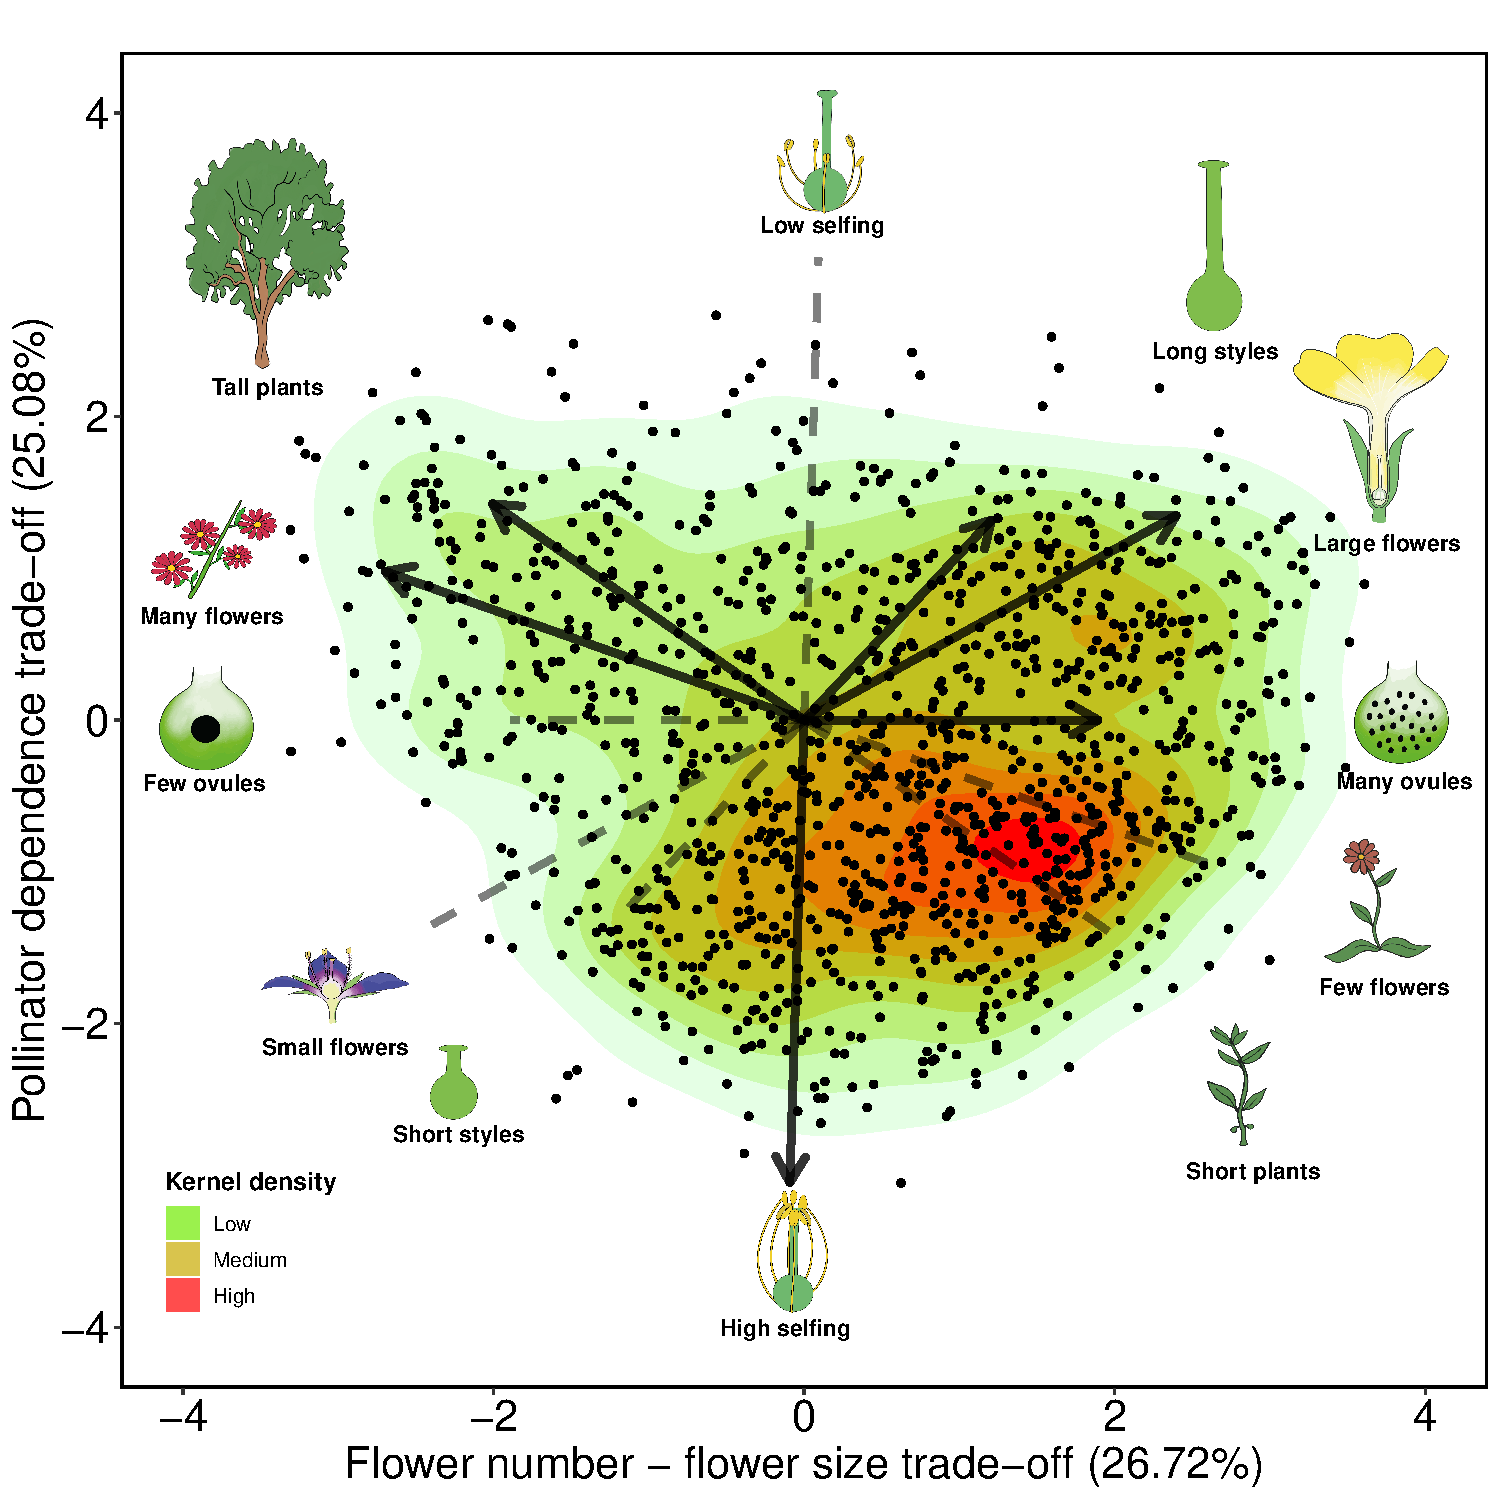
\includegraphics{output/figures/unnamed-chunk-1-1.pdf}
\caption{\label{fig:unnamed-chunk-1}\textbf{Fig. 1 \textbar{} Plant
life-history strategies.} Phylogenetically informed principal component
analysis (pPCA) of 1,236 plant species from 28 plant-pollinator networks
studies. The solid arrows indicate the direction of the different
quantitative traits (flower number, plant height, style length, flower
size, ovule number and level of autonomous selfing) across the two main
axes of trait variation. The length of the arrows indicate the weight of
the variables on each principal component and the labelled icons at
their end represent the extreme form of the trait continuum. The dashed
lines show the opposed direction of trait variation and the non-labelled
icons at their end illustrate the opposing extreme of the continuum.}
\end{figure}

We found that most categorical traits were statistically associated with
the first two axes of trait variation (Fig. 2 and Supplementary Table
S2). Flower symmetry, which was only associated with PC2 (Sum of squares
= 8.51, F-value = 14.72, \emph{P} \textless{} 0.01 ), and nectar
provision, which was independent of PC1 and PC2 (PC1: Sum of squares =
0.37, F-value = 0.29 , \emph{P} = 0.59; PC2: Sum of squares = 0.83,
F-value = 1.43, \emph{P} = 0.23) showed lack of statistical association.
In addition, we found with Tukey test statistical differences between
the different levels of categorical traits in the trait space
(Supplementary Fig. S7). Regarding self compatibility, we found larger
differences on PC2 (i.e., species with unisexual flowers that were self
incompatibile were statistically differentiated from species with
partial or full self compatibility; Supplementary Fig. S7a and Fig.
S7b). Life forms differed statistically across both axes of trait
variation and followed a gradient of larger life forms (trees and
shrubs) with higher pollinator dependence to smaller ones (herbs) with
lower pollinator dependence (Supplementary Fig. S7c and Fig. S7d).
Consequently, lifespan also followed this gradient but perennial and
short lived species only differed statistically on PC2 (Supplementary
Fig. S7e and Fig. S7f). Species with unisexual flowers (monoecious and
dioecious) were clustered on both extremes of the first two principal
components and had the highest pollinator dependence and highest number
of flowers (Supplementary Fig. S7g and Fig. S7h). Moreover, we found
that the campanulate and capitulum flower shapes were differentiated
from tube, papilionaceous, open and brush shapes in the trait space. The
former morphologies had larger flowers and greater pollinator
dependence, while the latter had higher flower number and greater
autonomous selfing (Supplementary Fig. S7i and Fig. S7j). Regarding
flower symmetry, zygomorphic flowers were associated with lower levels
of pollinator dependence, whereas actinomorphic flowers had higher
levels of pollinator dependence (Supplementary Fig. S7k and Fig. S7l).

\blandscape

\vspace*{-28mm}

\begin{figure}
\centering
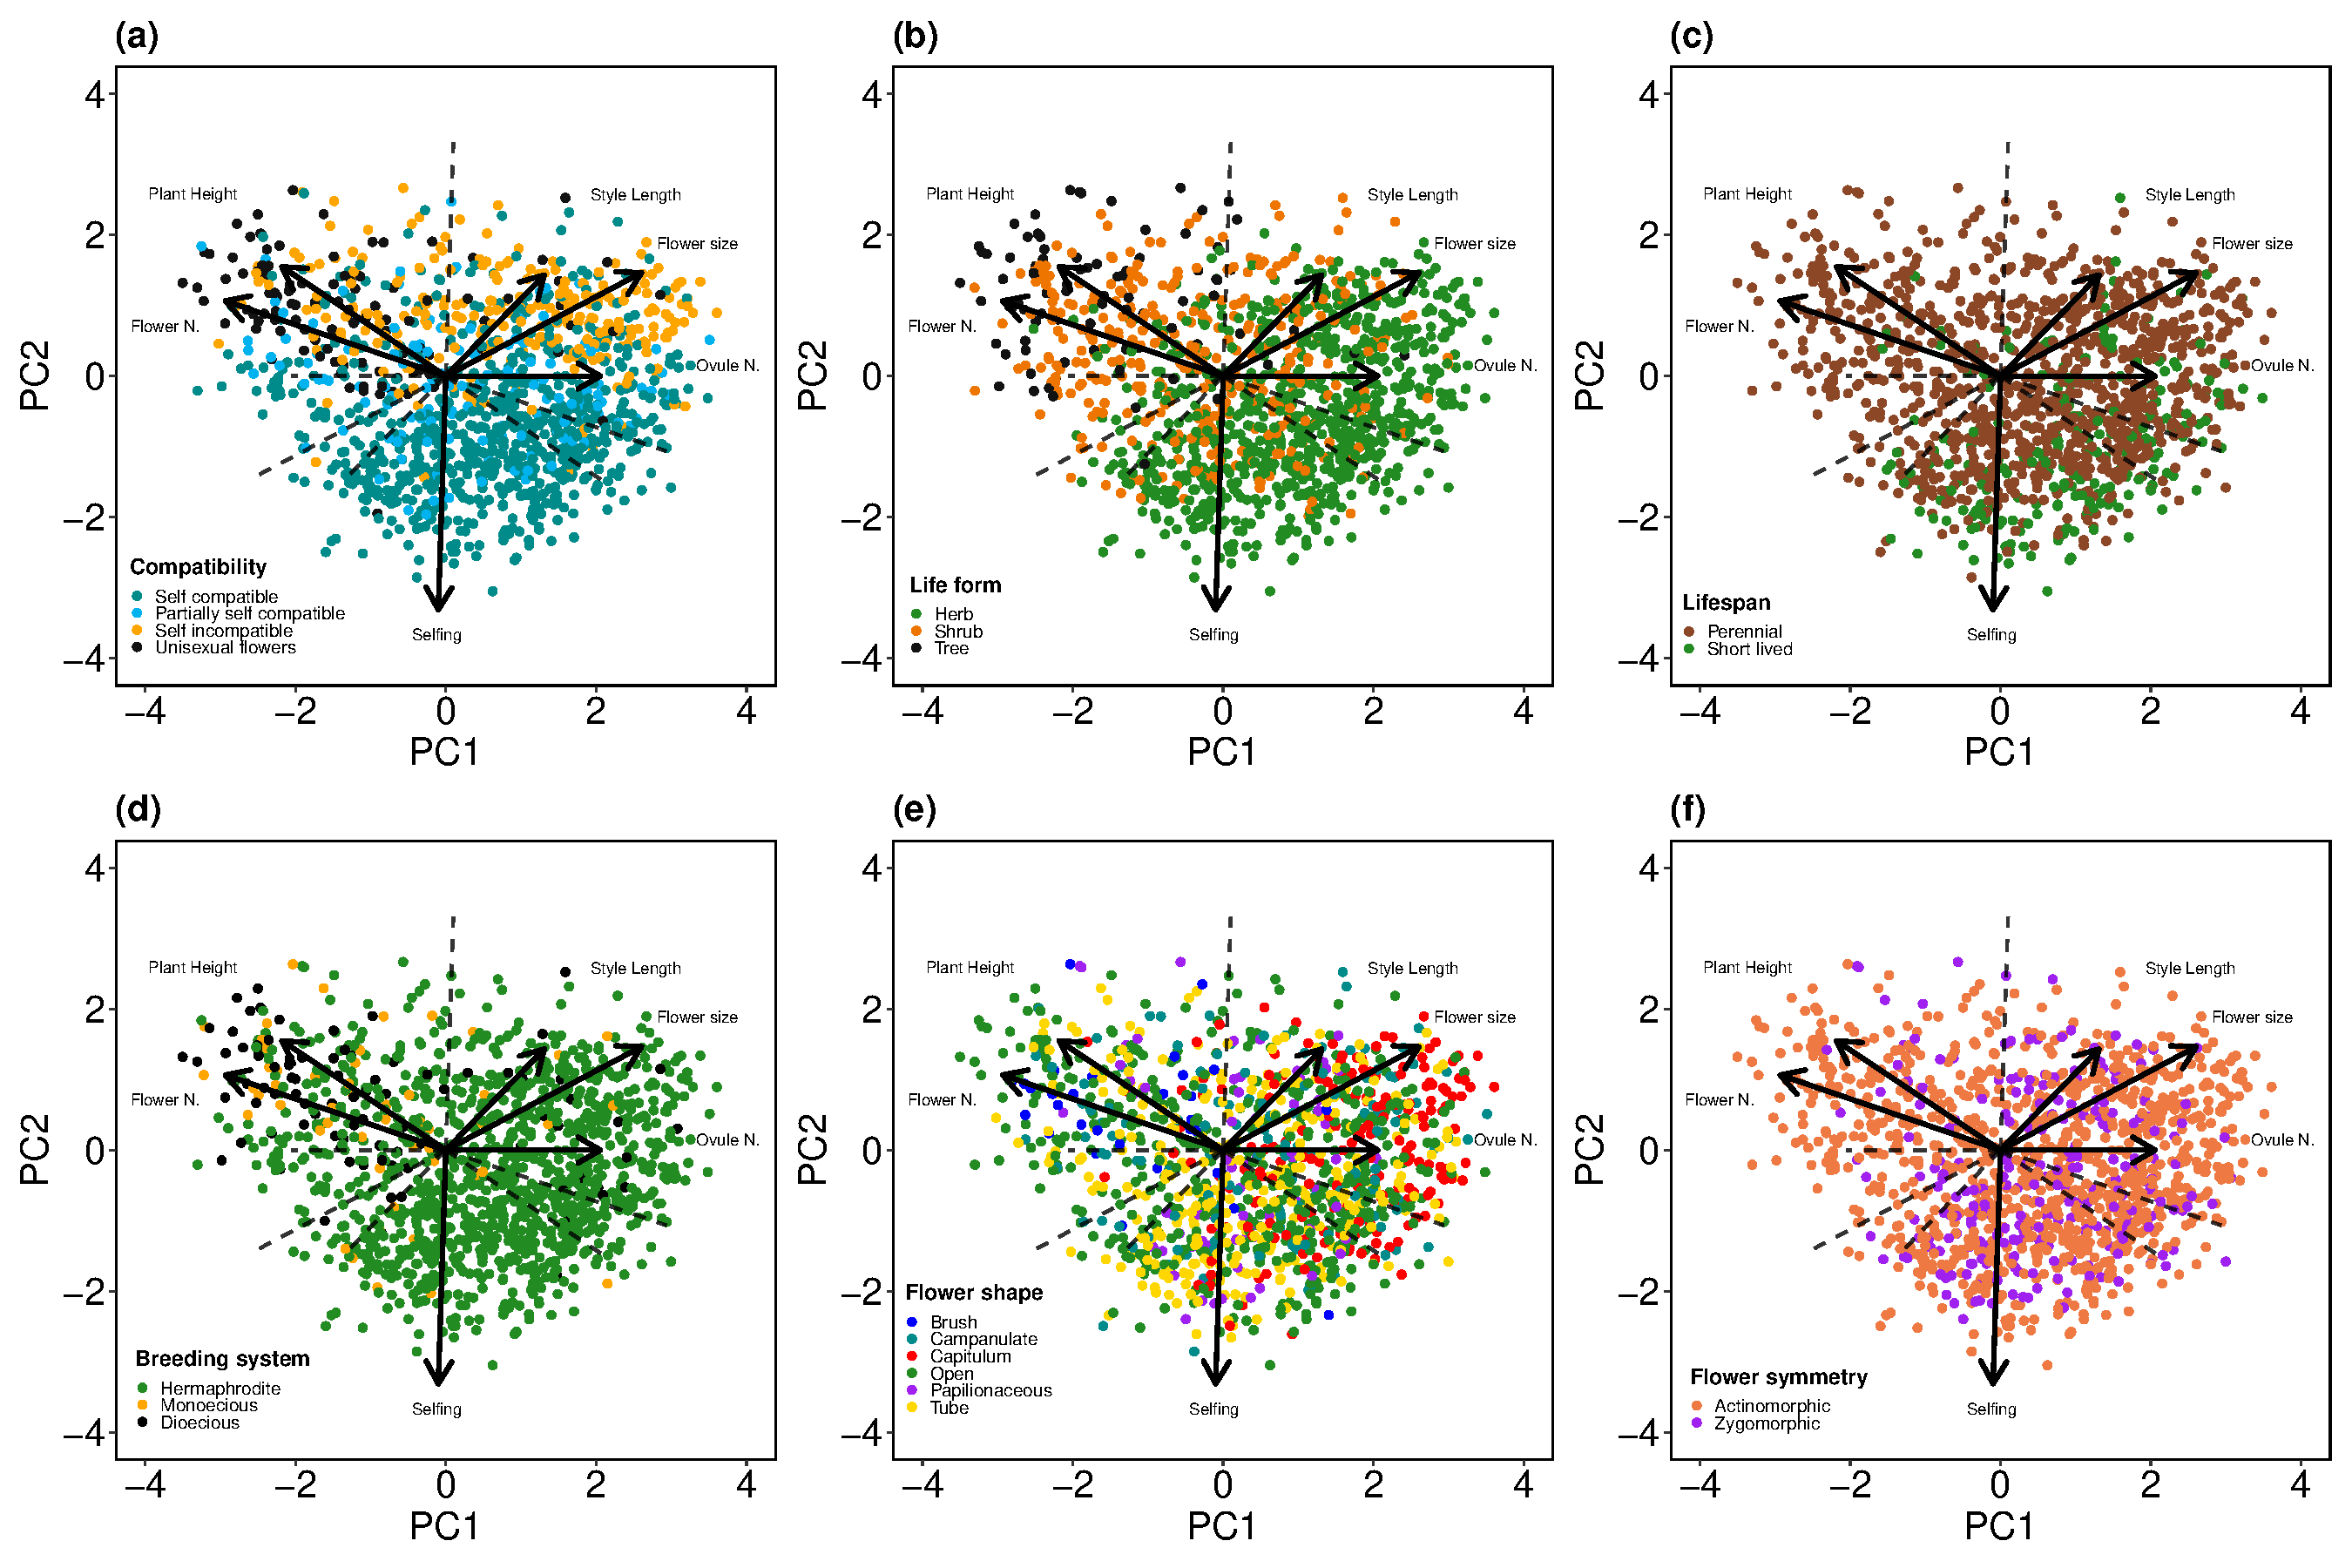
\includegraphics{output/figures/unnamed-chunk-2-1.pdf}
\caption{\label{fig:unnamed-chunk-2}\textbf{Fig. 2 \textbar{} Location of
the different qualitative traits on the trait space.} The panel is
composed by the traits that showed statistical association with the
first two axes of trait variation: compatibility system (a), life form
(b), lifespan (c), breeding system (d), flower shape (e) and flower
symmetry (f).}
\end{figure}

\elandscape

\vspace{5mm}

\textbf{Phylogenetic signal of traits.} We found a strong phylogenetic
signal (\emph{P} \textless{} 0.01) in all quantitative traits
(Supplementary Table S5). The traits that showed the highest
phylogenetic signal were ovule number (\(\lambda = 1\)), pollen grains
per flower (\(\lambda = 1\)) and plant height (\(\lambda = 0.96\)),
followed by flower length (\(\lambda = 0.75\)), flower width
(\(\lambda = 0.73\)), number of flowers per plant (\(\lambda = 0.69\))
and nectar concentration (\(\lambda = 0.65\)). The traits that showed a
moderate phylogenetic signal were inflorescence width
(\(\lambda = 0.57\)), style length (\(\lambda = 0.49\)) and autonomous
selfing (\(\lambda = 0.34\)). Finally, microliters of nectar per flower
showed the lowest phylogenetic signal of all traits
(\(\lambda = 0.14\)).

\textbf{Visitation patterns.} The main axes of trait variation explained
little of the overall visitation rates (\(conditional R2 = 0.31\);
\(marginal R2 = 0.06\)) but showed relevant trends when we explored the
interaction with the different floral visitors guilds (Fig. 3). All
floral visitors guilds visited plant species with higher pollinator
dependence more frequently (PC2; Fig. 3b and Fig. 3e). In addition, all
guilds other than Syrphids and Lepidoptera (i.e., all Hymenoptera,
non-Syrphidae-Diptera and Coleoptera) showed greater visitation rates on
species with small numerous flowers (PC1; Fig. 3a and Fig. 3d). On the
style length trade-off (PC3), Anthophila-Hymenoptera, Lepidoptera and
Non-Anthophila-Hymenoptera showed greater visitation rates on plant
species with larger styles and higher levels of selfing; while
Syrphidae, Non-Syrphidae-Diptera and Coleoptera showed higher visitation
rates on species with shorter styles and lower selfing (Fig. 3c and Fig.
3f). Furthermore, when running an additional model that separates the
most represented families of Anthophila-Hymenoptera (bees;
\(marginal R2 = 0.30\); \(conditional R2 = 0.03\)) showed that the
family Apidae was the main driver of the observed patterns
(Supplementary Fig. S8).

\blandscape

\begin{figure}
\centering
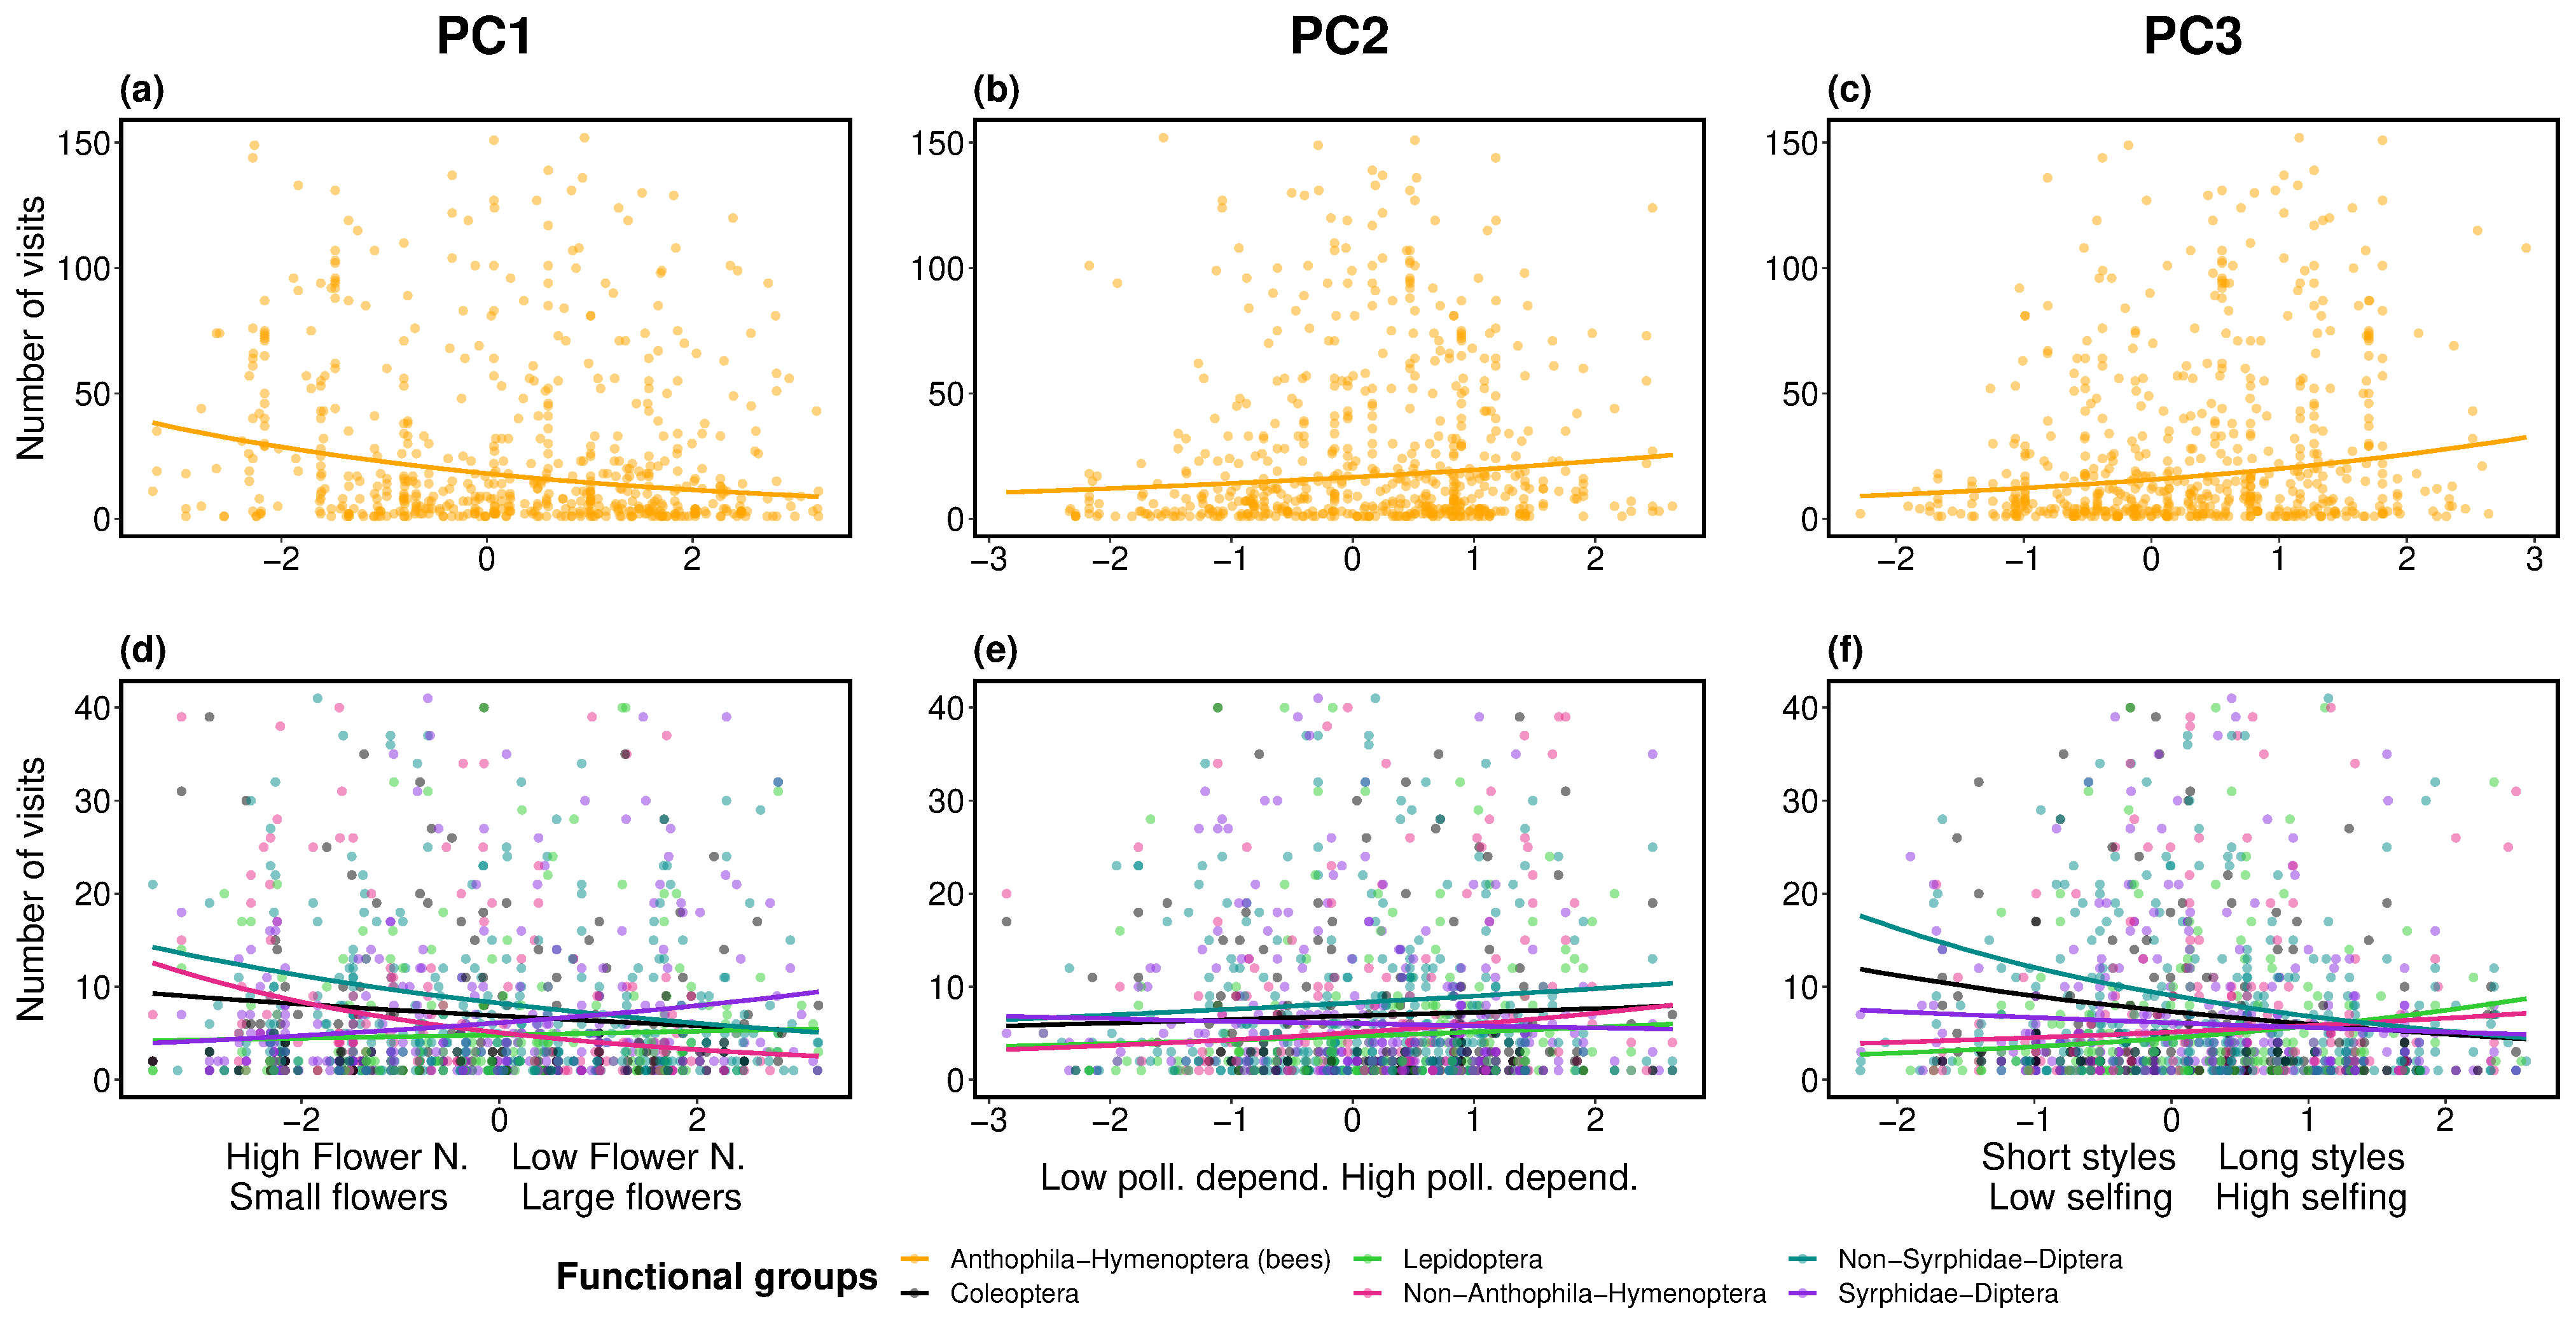
\includegraphics{output/figures/unnamed-chunk-3-1.pdf}
\caption{\label{fig:unnamed-chunk-3}\textbf{Fig. 3 \textbar{} Visitation
rates across the three main axes of trait variation.} Fitted posterior
estimates of the number of visits made by the different floral visitors
guilds in relation to PC1, PC2 and PC3. Bees (a, b and c) and the rest
of guilds (d, e and f) were plotted separately for visualization
purposes. In addition, we trimmed the plotting area that was over the
95th percentile to improve visualisation. PC1 represents the flower
number - flower size trade-off, PC2 represents the pollinator dependence
trade-off and PC3, the style length trade-off.}
\end{figure}

\elandscape

\textbf{Plant species functional roles.} The variance of the different
plant species level metrics was poorly explained by the three main axes
of trait variation (Supplementary Fig. S9; interaction frequency
\textasciitilde{} PCs, \(conditional R2 = 0.11\),
\(marginal R2 = 0.02\); normalized degree \textasciitilde{} PCs,
\(conditional R2 = 0.24\), \(marginal R2 = 0.02\); and, specialization
\textasciitilde{} PCs, \(conditional R2 = 0.37\),
\(marginal R2 = 0.03\)). Overall, the most notable trends were found on
PC1 and PC3 for interaction frequency and specialization. On the flower
number - flower size trade-off (PC1), interaction frequency was higher
for plant species with more flowers but was lower for plant species with
larger flowers. On PC1, specialization showed the opposite trend. On the
style length trade-off (PC3), interaction frequency was lower for plants
with shorter styles and lower autonomous selfing and higher for species
with longer styles and higher autonomous selfing. Again, specialization
showed the opposite trend to interaction frequency.

When we further investigate which combination of traits drive plant
network roles, we show that the regression tree for visitation frequency
was best explained by plant height, nectar concentration and style
length (Fig. 4a). Specifically, species taller than 3.9 m had the
highest interaction frequency, while species that were shorter than 3.9
m and had a nectar concentration lower than 16\% had the lowest
interaction frequency. Normalized degree was best explained by nectar
concentration, pollen grains per flower, plant height, flower width and
autonomous selfing (Fig. 4b). Species with a nectar concentration over
49\% had the highest levels of normalized degree, whereas species with
nectar concentration lower than 49\%, more than 21,000 pollen grains per
flower and height less than 0.78 m had the lowest normalized degree.
Finally, specialization was best explained by plant height, ovule
number, pollen grains per flower and autonomous selfing (Fig. 4c).
Overall, plant species with the highest specialization were shorter than
1.3 m, had more than 14,000 pollen grains per flower and autonomously
self-pollinated less than 11\% of their fruits. In contrast, species
taller or equal than 5.1 m and with lower than 14 ovules per flower had
the lowest specialization values.

\blandscape

\begin{figure}
\centering
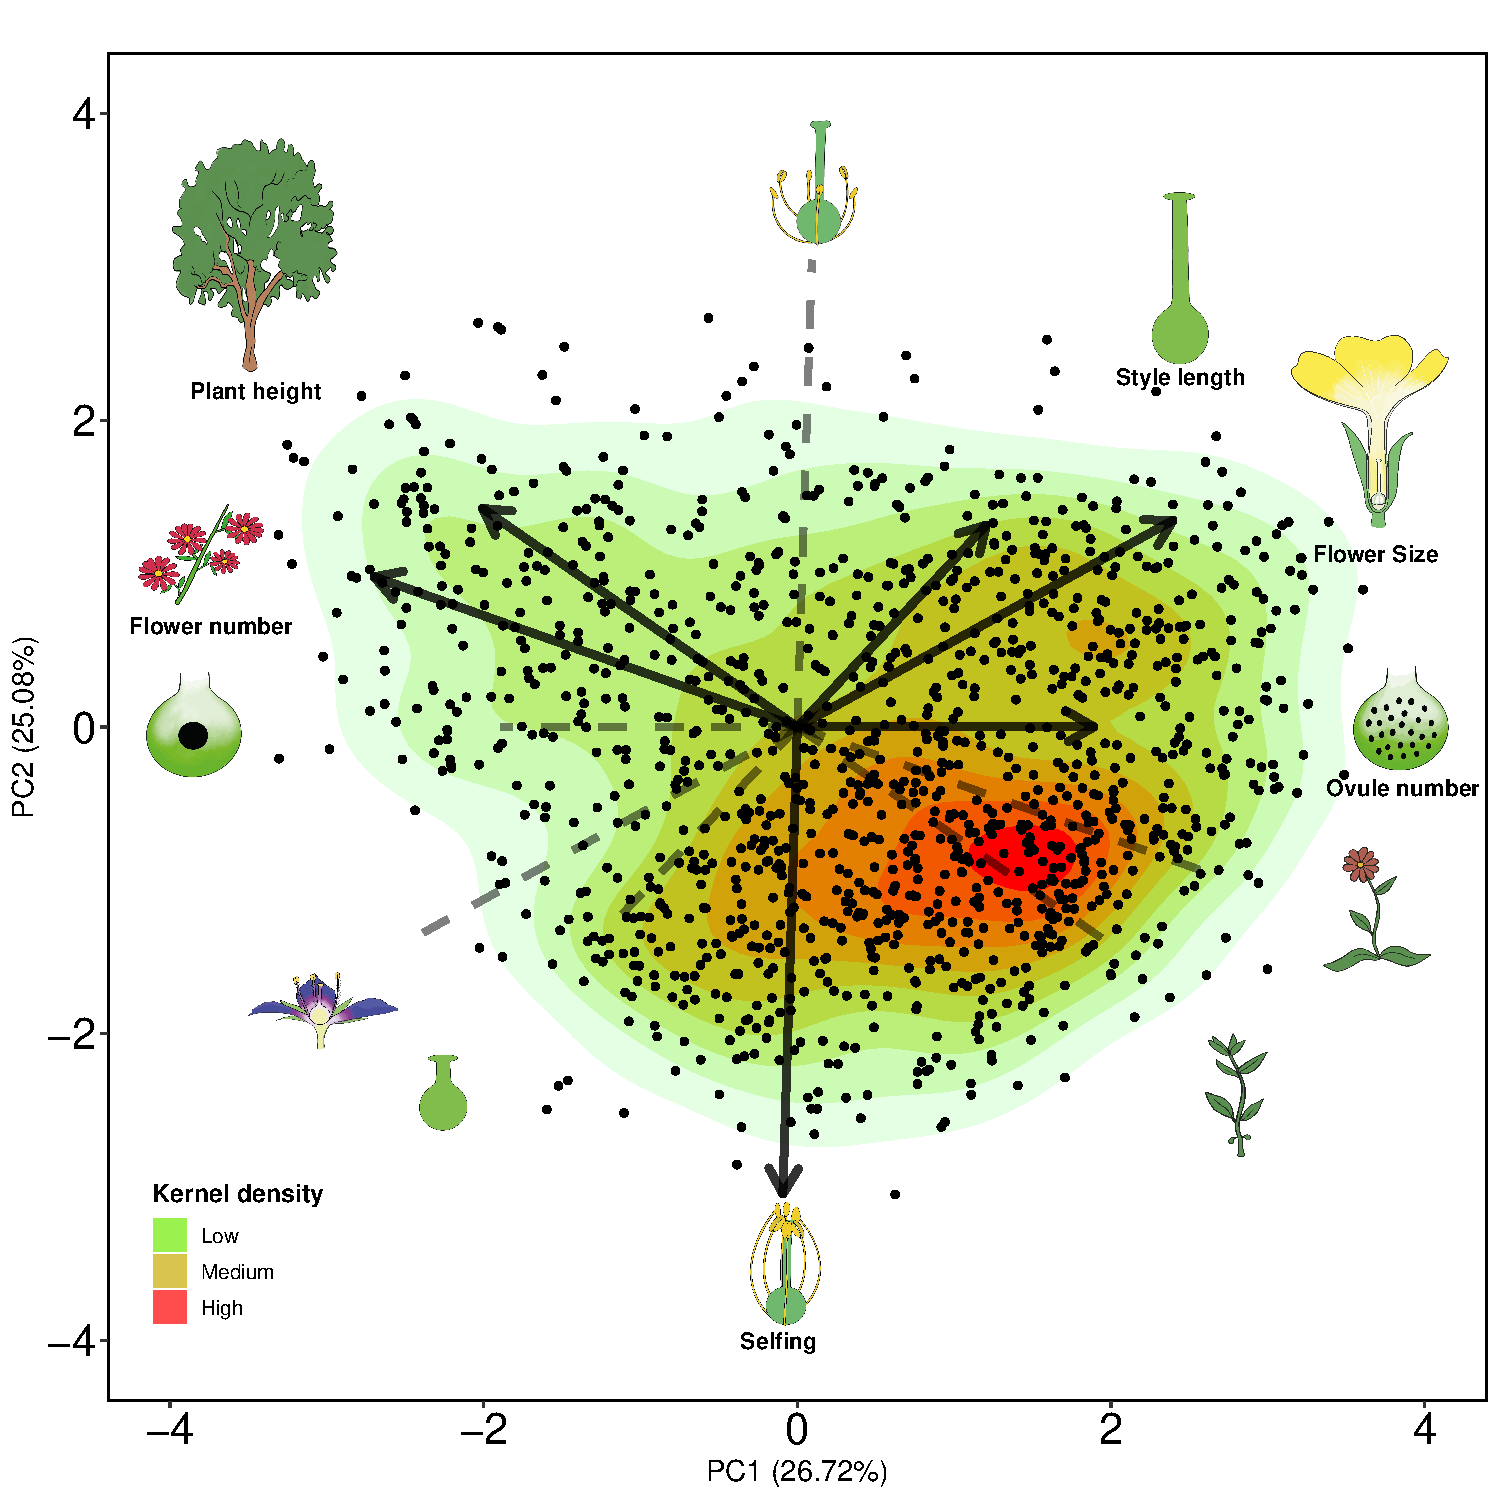
\includegraphics{output/figures/unnamed-chunk-4-1.pdf}
\caption{\label{fig:unnamed-chunk-4}\textbf{Fig. 4 \textbar{} contribution
of traits in plant's network roles.} Regression tree analysis of
interaction frequency (log-transformed), normalized degree and
specialization for the subset of species with quantitative data for
pollen and nectar traits. The superior value inside the node indicates
the mean value of the different species-level metric and the lower
value, the percentage of species that are considered in each node. Thus,
the top node has the mean value of the named trait for the 100\% of
species. Each node has a yes/no question and when the condition is
fulfilled, the branch turns to the `yes' direction and when not, to the
`no' direction. This rationale is followed in all the regression trees
as indicated in the first branch division of the topmost node of each
tree.}
\end{figure}

\elandscape

\section{DISCUSSION}\label{discussion}

Here, we show that plant species exhibit clear trade-offs in their
floral, reproductive and vegetative traits. These trade-offs are
differentiated on three main axes of trait variation: (i) flower number
- flower size, (ii) pollinator dependence and (iii) style length.
Although these axes of trait variation did not explain overall
visitation rates, we found that plant life strategies were clearly
associated with different floral visitors guilds. Interestingly, pollen
and nectar related traits were better than all other traits for
characterizing plant species functional roles within their interaction
networks.

Over 50\% of plant trait variation was captured by the flower number -
flower size and pollinator dependence trade-offs. Variation in these two
axes of trait variation appears to be associated with the commonly
described `fast-slow continuum' in
plant\textsuperscript{\protect\hyperlink{ref-salguero2016}{8}} and
animal\textsuperscript{\protect\hyperlink{ref-healy2019}{34}}
life-history strategies as indicated by the different floral and
reproductive traits associated with plant height, life form and
lifespan. The `slow' part of the continuum (i.e., tall trees and shrubs)
had plant species with many flowers, few ovules, higher pollinator
dependence, greater occurrence of self-incompatibility and more complex
breeding systems (e.g., monoecious and dioecious species). In contrast,
species that employed the `fast' strategy (i.e., short herbs), had fewer
flowers, more ovules, greater occurrence of self compatibility and lower
pollinator dependence. Further, on the first two axes of trait
variation, we found additional support for the positive association
already described in a previous study between outcrossing rate and
floral
display\textsuperscript{\protect\hyperlink{ref-goodwillie2010}{24}}.
This trend was further confirmed when looking at the specific
correlation between floral display and autonomous selfing for our
dataset (see Supplementary Fig. S10).

Despite the low predictive power of the main axes of trait variation on
overall visitation patterns, we found commonalities among and within
floral visitors guilds across these axes that indicate the influence of
life-history strategies on floral visitation rate. For example, all
guilds showed an increasing trend of visitation on plant species with
higher pollinator dependence, which were also associated with larger
floral displays and greater pollen quantities (Fig. 1 and Supplementary
Fig. S6). This trend is consistent with previous plant-pollinator
studies that show higher visitation rates on species that make greater
reproductive
investment\textsuperscript{\protect\hyperlink{ref-hegland2005}{35}--\protect\hyperlink{ref-kaiser2014}{37}}.
In regard to the flower number - flower size and style length
trade-offs, different guilds showed contrasting visitation rates, which
could be associated with different pollination syndromes at a
macroecological scale. For instance, the guilds of bees and syrphids
were clearly associated with opposing life-strategies on PC1 and PC3
(Fig. 3) indicating a possible niche partitioning among these two
guilds\textsuperscript{\protect\hyperlink{ref-palmer2003}{38},\protect\hyperlink{ref-phillips2020}{39}}.
However, these plant-pollinator associations do not account for some of
the traits (i.e., pollen and nectar quantity) that had greater relevance
on the species network roles (Fig. 4) because of insufficient data
availability and lack of pollinator efficiency measurements for more
complete descriptions of the pollination
syndromes\textsuperscript{\protect\hyperlink{ref-dellinger2020}{13}}. In
any case, it is worth noting that this general pattern emerges in
field-measured plant-pollinator networks, where other local factors such
as species relative abundances, will surely explain part of the observed
variability\textsuperscript{\protect\hyperlink{ref-bartomeus2016}{12},\protect\hyperlink{ref-vazquez2007}{40},\protect\hyperlink{ref-encinas2012}{41}}.

To conclude, we provide the first description of plant floral and
reproductive trade-offs using a large global dataset of plant traits and
interactions with floral visitors. This allowed us to identify the major
reproductive strategies of flowering plants and how plant life
strategies determine their interaction with floral visitor guilds.
Although the percentage of explained variation found with the first two
axes (\textasciitilde{}50\%) is lower than other studies that have
evaluated life histories with vegetative
traits\textsuperscript{\protect\hyperlink{ref-diaz2016}{18},\protect\hyperlink{ref-carmona2021}{19}},
this percentage is consistent with the largest and most recent study
that have characterized life strategies with both vegetative and
reproductive (i.e., semelparity and iteroparity)
traits\textsuperscript{\protect\hyperlink{ref-salguero2016}{8}}. Future
work needs to integrate these floral and reproductive compromises with
the already described vegetative and physiological
trade-offs\textsuperscript{\protect\hyperlink{ref-diaz2016}{18}} to
create a more comprehensive spectra of trait
variation\textsuperscript{\protect\hyperlink{ref-roddy2021}{10}}.
Further, the varying level of phylogenetic signal among traits deserves
further attention to understand evolutionary changes on mating and
flower morphology in response to
pollinators\textsuperscript{\protect\hyperlink{ref-gervasi2017}{42},\protect\hyperlink{ref-mackin2021}{43}}.
Finally, a more complete description of the macroecological patterns of
plant-pollinator interactions including unrepresented areas of the
world\textsuperscript{\protect\hyperlink{ref-poisot2021}{44}} and traits
that have been largely ignored (e.g., floral rewards and plant mating
system) are needed to progress in our understanding of the global
patterns in plant-pollinator interactions.

\section{MATERIALS AND METHODS}\label{materials-and-methods}

\textbf{Plant-pollinator network studies.} We selected 28 studies from
18 different countries that constituted a total of 64 plant-pollinator
networks. These studies recorded plant-pollinator interactions in
natural systems and were selected so that we had broad geographical
representation. Although these studies differ in sampling effort and
methodology, all studies provided information about plant-pollinator
interactions (weighted and non-weighted), which we used to build a
database of plant species that are likely to be animal pollinated. Many
of these networks are freely available either as published
studies\textsuperscript{\protect\hyperlink{ref-carvalheiro2014}{3},\protect\hyperlink{ref-fortuna2010}{45}}
or available in online archives (e.g., `The Web of
Life'\textsuperscript{\protect\hyperlink{ref-fortuna2010}{45}} and
`Mangal'\textsuperscript{\protect\hyperlink{ref-poisot2016}{46}}. In
total, our network dataset (see Supplementary Table S1) constituted 60
weighted (interaction frequency) and 4 unweighted (presence/absence of
the interaction) networks, each sampled at a unique location and year,
as well as eight meta-webs where interactions were pooled across several
locations and multiple years.

\textbf{Taxonomy of plants and pollinators.} All species names, genera,
families and orders were retrieved and standardized from the taxonomy
data sources NCBI (\url{https://www.ncbi.nlm.nih.gov/taxonomy}) for
plants and ITIS (\url{https://www.itis.gov/}) for pollinators, using the
R package
\emph{taxize}\textsuperscript{\protect\hyperlink{ref-chamberlain2020}{47}}.
We filled the `not found' searches manually using
\url{http://www.theplantlist.org/} and \url{http://www.mobot.org/} for
plants and \url{http://www.catalogueoflife.org/} for floral visitors.

\textbf{Functional traits.} We selected 20 different functional traits
based on their relevance to plant reproduction and data availability
(Table 1). These included twelve quantitative and eight categorical
traits belonging to three broader trait groupings (13 floral, 4
reproductive and 3 vegetative). For each plant species, we undertook an
extensive literature and online search across a wide range of resources
(plant databases, online floras, books, journals and images). From a
total of 30,120 cells (20 columns × 1,506 species) we were able to fill
24,341 cells (80.8\% of the dataset, see Supplementary Fig. S1 for
missing values information for each trait).

\textbf{Phylogenetic Distance.} We calculated the phylogenetic distance
between different plant species using the function \emph{get\_tree} from
the package \emph{rtrees} (\url{https://github.com/daijiang/rtrees}),
which downloads phylogenetic distances from the extended R
implementation of the Open Tree of
Life\textsuperscript{\protect\hyperlink{ref-smith2018}{48},\protect\hyperlink{ref-jin2019}{49}}.

\singlespacing

\begin{table}

\caption{\label{tab:unnamed-chunk-5}\textbf{Table 1 | Quantitative and categorical traits used in this study.}}
\centering
\fontsize{10}{12}\selectfont
\begin{tabu} to \linewidth {>{}c>{\raggedright}X>{}c>{\centering}X>{\raggedright}X}
\toprule
\multicolumn{2}{c}{\textbf{Quantitative traits}} & \multicolumn{3}{c}{\textbf{Categorical traits}} \\
\cmidrule(l{3pt}r{3pt}){1-2} \cmidrule(l{3pt}r{3pt}){3-5}
\textbf{Type} & \textbf{Traits} & \textbf{Type} & \textbf{Traits} & \textbf{Categories}\\
\midrule
\textbf{Vegetative} & Plant height (m) & \textbf{Vegetative} & Lifepan & \makecell[l]{Short-lived \\ Perennial}\\
\addlinespace
\textbf{Floral} & Flower width (mm) & \textbf{Vegetative} & Life form & \makecell[l]{Herb \\ Shrub \\ Tree}\\
\addlinespace
\textbf{Floral} & Flower length (mm) & \textbf{Floral} & Flower shape & \makecell[l]{Brush \\ Campanulate \\ Capitulum \\ Open \\ Papilionaceous \\ Tube}\\
\addlinespace
\textbf{Floral} & Inflorescence width (mm) & \textbf{Floral} & Flower symmetry & \makecell[l]{Actinomorphic \\ Zygomorphic}\\
\addlinespace
\textbf{Floral} & Style length (mm) & \textbf{Floral} & Nectar & \makecell[l]{Presence \\ Absence}\\
\addlinespace
\textbf{Floral} & Ovules per flower & \textbf{Reproductive} & Autonomous selfing & \makecell[l]{None \\ Low \\ Medium \\ High}\\
\addlinespace
\textbf{Floral} & Flowers per plant & \textbf{Reproductive} & Compatibility system & \makecell[l]{Self-incomp. \\ Part. self-comp. \\ Self-comp.}\\
\addlinespace
\textbf{Floral} & Nectar ($\mu$l) & \textbf{Reproductive} & Breeding system & \makecell[l]{Hermaphrodite \\ Monoecious \\ Dioecious}\\
\addlinespace
\textbf{Floral} & Nectar (mg) & \textbf{} &  & \\
\addlinespace
\textbf{Floral} & Nectar concentration ($\%$) & \textbf{} &  & \\
\addlinespace
\textbf{Floral} & Pollen grains per flower & \textbf{} &  & \\
\addlinespace
\textbf{Reproductive} & Autonomous selfing (fruit set) & \textbf{} &  & \\
\bottomrule
\end{tabu}
\end{table}

\doublespacing

\textbf{Data Imputation.} Trait missing values were imputed with the
function
\emph{missForest}\textsuperscript{\protect\hyperlink{ref-stekhoven2012}{50}}
which allows imputation of data sets with continuous and categorical
variables. We accounted for the phylogenetic distance among species on
the imputation process by including the eigenvectors of a principal
component analysis of the phylogenetic distance (PCoA) which has been
shown to improve the performance of
\emph{missForest}\textsuperscript{\protect\hyperlink{ref-penone2014}{51}}.
To extract the eigenvectors, we used the function \emph{PVRdecomp} from
the package
\emph{PVR}\textsuperscript{\protect\hyperlink{ref-santos2018}{52}} based
on a previous conceptual framework that considers phylogenetic
eigenvectors\textsuperscript{\protect\hyperlink{ref-diniz-filho2012}{53}}.
Although the variable of autonomous selfing had a high percentage of
missing values (68\%), we were able to solve this by back transforming
the qualitative column of autonomous selfing to numerical. The
categories of `none', `low', `medium' and `high' were converted to
representative percentages of each category 0\%, 13\%, 50.5\% and 88\%
respectively. This reduced the percentage of missing values for this
column from 68\% to 35\% and allowed the imputation of this variable.
However, we were unable to include nectar and pollen traits on the
imputation process because of the high percentage of missing values
(Supplementary Fig. S1). Hence, the imputed dataset had 1,506 species,
seven categorical and eight numerical variables and 5.79\% of missing
values. Further, we conducted an additional imputation on the filtered
raw data by filled cells of either pollen grains per flower or
microlitres of nectar. This subset comprised 755 species, 8.01\% missing
values and all traits but milligrams of nectar (\textasciitilde{}50\% of
missing values) were included in the imputation process.

\textbf{Plant strategies.} We explored the trade-offs between different
quantitative plant functional traits with a phylogenetically informed
Principal Component Analysis (pPCA). We did not include the quantitative
variables of flower length and inflorescence width because they were
highly and moderately correlated to flower width respectively (Pearson's
correlation = 0.72, \emph{P} \textless{} 0.01 and Pearson's correlation
= 0.36, \emph{P} \textless{} 0.01 respectively), and thus we avoided
overemphasizing flower size on the spectrum of trait variation. Although
qualitative traits were not included in the dimensionality reduction
analysis, we also investigated the association of the different
qualitative traits with the main axes of trait variation. Prior to the
analyses, we excluded outliers and standardized the data. Due to the
high sensitivity of dimensionality reduction to outliers, we excluded
values within the 2.5th--97.5th percentile
range\textsuperscript{\protect\hyperlink{ref-legendre2012}{54}}, and
thus our final dataset had 1,236 species. Then, we log transformed the
variables to reduce the influence of outliers and z-transformed (X= 0,
SD=1) so that all variables were within the same numerical range. We
performed the pPCA using the function \emph{phyl.pca} from the package
\emph{phytools}\textsuperscript{\protect\hyperlink{ref-revell2012}{55}}
with the method lambda (\(\lambda\)) that calculates the phylogenetic
correlation between 0 (phylogenetic independence) and 1 (shared
evolutionary history) and we implemented the mode covariance because
values for each variables were on the same scale following
transformation\textsuperscript{\protect\hyperlink{ref-abdi2010}{56}}.
Moreover, to corroborate that our imputation of missing values did not
affect our results, we conducted a pPCA on the full dataset without
missing values (see Supplementary Fig. S2). We found little difference
between the explained variance with the imputed dataset (51.08\%) and
the dataset without missing values (52.87\%). In addition, the loadings
on each principal component had a similar contribution and correlation
patterns, with the exception of plant height which showed slight
variations between the imputed and non-imputed dataset. Finally, we
conducted an additional phylogenetic informed principal component
analysis for the subset of species with pollen and nectar quantity. For
this, we included all quantitative traits considered in the main pPCA
plus pollen grains and microlitres of nectar per flower.

\textbf{Phylogenetic signal of traits.} We calculated the phylogenetic
signal of the different quantitative traits on the imputed dataset with
the full set of species (N = 1,506) with the package \emph{phytools}
version
\emph{0.7-70}\textsuperscript{\protect\hyperlink{ref-revell2012}{55}}
and we used Pagel's \(\lambda\) as a measurement of the phylogenetic
signal. However, for pollen and nectar traits, phylogenetic signal was
calculated only on the subset of species that had quantitative
information for these traits (N = 755).

\textbf{Networks analyses.} Analyses were conducted on the subset of 60
weighted networks with interaction frequency sampled in a unique
flowering season and site, which included 556 plant and 1,126 pollinator
species. In total, our weighted network dataset (excluding meta-webs)
included 2,256 interactions of Anthophila-Hymenoptera (i.e., bees) with
plants, 1,768 non-Syrphidae-Diptera interactions, 845 Syrphidae
interactions, 437 Lepidoptera interactions, 432 Coleoptera interactions
and 362 non-Anthophila-Hymenoptera interactions. Although floral
visitors are not always pollinators and the frequency of visits does not
consider each pollinator species
efficiency\textsuperscript{\protect\hyperlink{ref-ballantyne2015}{57}},
visitation rate provides valuable information of the contribution of
floral visitors to
pollination\textsuperscript{\protect\hyperlink{ref-vazquez2005}{58},\protect\hyperlink{ref-vazquez2012}{59}}.
Sampling methods varied across networks but this was accounted for in
analyses by considering them in the random effects of the modelling
process. All analyses were conducted in R version \emph{4.0.3}.

\textbf{Visitation patterns.} We used Bayesian modelling (see below for
details) to explore the effect of floral visitors groups and the main
axes of trait variation (pPCA with imputed dataset) on floral visits per
plant species. For this, we divided floral visitors into six main guilds
that differ in life form, behaviour and are likely to play a similar
ecological role: (i) Hymenoptera-Anthophila (bees), (ii)
Hymenoptera-non-Anthophila (non-bee Hymenoptera), (iii)
Syrphidae-Diptera, (iv) non-Syrphidae-Diptera, (v) Lepidoptera and (vi)
Coleoptera. Moreover, because Hymenoptera-Anthophila was the most
represented group with 2,256 records and had the highest frequency of
visits of all groups, we also explored the visitation rate of the main
Hymenoptera-Anthophila families (Andrenidae, Apidae, Colletidae,
Halictidae and Megachilidae) on the trait space. In addition, we found
that \emph{Apis mellifera} was the floral visitor with the largest
proportion of records counted (7.55\% of the total). This finding is
consistent with previous research showing that \emph{A. mellifera} was
the most frequent floral visitor in a similar dataset of 80
plant-pollinator networks in natural
ecosystems\textsuperscript{\protect\hyperlink{ref-hung2018}{60}}. Hence,
to control for the effect of \emph{A. mellifera} on the observed
visitation patterns of bees, we conducted an analogous analysis
excluding \emph{A. mellifera}. We found that \emph{A. mellifera}, was
partly driving some of the observed trends on PC1 (Supplementary Fig.
S3). However, we did not detect major differences on PC2 and PC3.

We implemented Bayesian generalized linear mixed models using the R
package
\emph{brms}\textsuperscript{\protect\hyperlink{ref-burkner2017}{61}}. We
modelled the frequency of visits as a function of the main axes of plant
trait variation and their interactions with floral visitor functional
groups (Visits \textasciitilde{} PC1 x FGs + PC2 x FGs + PC3 x FGs).
Because we were interested in possible differences in the visitation
patterns among floral visitors groups to plants with different
strategies, we included interactions between the main axes of trait
variation (PC1, PC2 and PC3) and the floral visitor guilds. In this
model, we added a nested random effect of networks nested within the
study system to capture the variation in networks among studies and
within networks. Moreover, we included the phylogenetic covariance
matrix as a random factor due to the possible shared evolutionary
histories of species and therefore lack of independence across them. We
specified this model with a zero inflated negative binomial distribution
and weakly informative priors from the brms function. We run this model
for 3,000 iterations and with previous 1,000 warm up iterations. We set
delta (\(\Delta\)) to 0.99 to avoid divergent transitions and visualized
the posterior predictive checks with the function \emph{pp\_check} using
the \emph{bayesplot}
package\textsuperscript{\protect\hyperlink{ref-gabry2019}{62}}.

\textbf{Plant species functional roles.} We investigated whether
different quantitative traits determined plant species functional roles
using Bayesian modelling and regression trees. For this, we selected
simple and complementary species-level network metrics commonly applied
in bipartite network
studies\textsuperscript{\protect\hyperlink{ref-dormann2008}{63}} with a
straightforward ecological interpretation relevant to our research
goals. The different plant species-level metrics were: (i) sum of visits
per plant species; (ii) normalized degree, calculated as the number of
links per plant species divided by the total possible number of
partners; and (iii)
specialization\textsuperscript{\protect\hyperlink{ref-bluthgen2006}{64}},
which measures the deviation of an expected random choice of the
available interaction partners and ranges between 0 (maximum
generalization) and 1 (maximum specialization). Normalized degree and
specialization were calculated with the \emph{specieslevel} function
from the R package
\emph{bipartite}\textsuperscript{\protect\hyperlink{ref-dormann2008}{63}}.

First, we modelled the distinct plant species metrics (sum of visits,
normalized degree and plant specialization) as a function of the three
main axes of trait variation (plant species level metric
\textasciitilde{} PC1 + PC2 + PC3). For each response variable (i.e.,
each plant species level metric), we used different distribution
families (zero inflated negative binomial for the sum of visits, weibull
for normalized degree and zero one inflated beta for specialization).
Finally, we used the same random factors, model settings and conducted
the same posterior predictive checks for each model as detailed above in
the `visitation patterns section'.

Second, to better understand these complex trait relationships, we used
regression trees. Regression trees are recursive algorithms which can
detect complex relationships among predictors and allow identification
of the relevance of specific trait combinations on species functional
roles. We focused exclusively on quantitative traits because almost all
categorical traits were statistically associated with the first two axes
of trait variation (Supplementary Table S2). We conducted this analysis
using the \emph{rpart}
package\textsuperscript{\protect\hyperlink{ref-therneau2015}{65}}
version \emph{4.1-15} with method \emph{`anova'} with a minimum of 50
observations per terminal node and we used the \emph{rpart.plot}
package\textsuperscript{\protect\hyperlink{ref-milborrow2015}{66}}
version \emph{3.0.9} to plot the regression trees. We considered the
species level indices as response variables (interaction frequency,
normalized degree and specialization) and we performed one regression
tree per metric using the different quantitative traits as predictors.
We calculated two regression trees per plant species-level metric, one
for the full set of species and another for the subset of species for
which we had pollen and nectar traits. We focused on regression trees
that included floral rewards because they consistently showed pollen and
nectar traits as being the best for explaining the different
species-level metrics (see Supplementary Fig. S4).

\section{References}\label{references}

\hypertarget{refs}{}
\hypertarget{ref-barrett2002}{}
1. Barrett, S. C. H. The evolution of plant sexual diversity. \emph{Nat.
Rev. Genet.} \textbf{3}, 274--284 (2002).

\hypertarget{ref-schiestl2013}{}
2. Schiestl, F. P. \& Johnson, S. D. Pollinator-mediated evolution of
floral signals. \emph{Trends Ecol. Evol.} \textbf{28}, 307--315 (2013).

\hypertarget{ref-carvalheiro2014}{}
3. Carvalheiro, L. G. \emph{et al.} The potential for indirect effects
between co-flowering plants via shared pollinators depends on resource
abundance, accessibility and relatedness. \emph{Ecol. Lett.}
\textbf{17}, 1389--1399 (2014).

\hypertarget{ref-baude2016}{}
4. Baude, M. \emph{et al.} Historical nectar assessment reveals the fall
and rise of floral resources in britain. \emph{Nature} \textbf{530},
85--88 (2016).

\hypertarget{ref-munoz2016}{}
5. Munoz, F., Violle, C. \& Cheptou, P.-O. CSR ecological strategies and
plant mating systems: Outcrossing increases with competitiveness but
stress-tolerance is related to mixed mating. \emph{Oikos} \textbf{125},
1296--1303 (2016).

\hypertarget{ref-moeller2017}{}
6. Moeller, D. A. \emph{et al.} Global biogeography of mating system
variation in seed plants. \emph{Ecol. Lett.} \textbf{20}, 375--384
(2017).

\hypertarget{ref-grossenbacher2017}{}
7. Grossenbacher, D. L. \emph{et al.} Self-compatibility is
over-represented on islands. \emph{New Phytol.} \textbf{215}, 469--478
(2017).

\hypertarget{ref-salguero2016}{}
8. Salguero-Gómez, R. \emph{et al.} Fast-slow continuum and reproductive
strategies structure plant life-history variation worldwide.
\emph{Proceedings of the National Academy of Sciences of the United
States of America} \textbf{113}, 230--235 (2016).

\hypertarget{ref-ruger2018}{}
9. Rüger, N. \emph{et al.} Beyond the fastSlow continuum: Demographic
dimensions structuring a tropical tree community. \emph{Ecol. Lett.}
\textbf{21}, 1075--1084 (2018).

\hypertarget{ref-roddy2021}{}
10. Roddy, A. B. \emph{et al.} Towards the flower economics spectrum.
\emph{New Phytol.} \textbf{229}, 665--672 (2021).

\hypertarget{ref-fenster2004}{}
11. Fenster, C. B., Armbruster, W. S., Wilson, P., Dudash, M. R. \&
Thomson, J. D. Pollination Syndromes and Floral Specialization.
\emph{Annual Review of Ecology, Evolution, and Systematics} \textbf{35},
375--403 (2004).

\hypertarget{ref-bartomeus2016}{}
12. Bartomeus, I. \emph{et al.} A common framework for identifying
linkage rules across different types of interactions. \emph{Functional
Ecology} \textbf{30}, 1894--1903 (2016).

\hypertarget{ref-dellinger2020}{}
13. Dellinger, A. S. Pollination syndromes in the 21st century: Where do
we stand and where may we go? \emph{New Phytol.} \textbf{228},
1193--1213 (2020).

\hypertarget{ref-tur2013}{}
14. Tur, C., Castro-Urgal, R. \& Traveset, A. Linking Plant
Specialization to Dependence in Interactions for Seed Set in Pollination
Networks. \emph{PLoS ONE} \textbf{8}, e78294 (2013).

\hypertarget{ref-devaux2014}{}
15. Devaux, C., Lepers, C. \& Porcher, E. Constraints imposed by
pollinator behaviour on the ecology and evolution of plant mating
systems. \emph{Journal of Evolutionary Biology} \textbf{27}, 1413--1430
(2014).

\hypertarget{ref-kattge2011}{}
16. Kattge, J. \emph{et al.} TRY a global database of plant traits.
\emph{Global Change Biology} \textbf{17}, 2905--2935 (2011).

\hypertarget{ref-salguero2015}{}
17. Salguero-Gómez, R. \emph{et al.} The compadre Plant Matrix Database:
An open online repository for plant demography. \emph{Journal of
Ecology} \textbf{103}, 202--218 (2015).

\hypertarget{ref-diaz2016}{}
18. Díaz, S. \emph{et al.} The global spectrum of plant form and
function. \emph{Nature} \textbf{529}, 167--171 (2016).

\hypertarget{ref-carmona2021}{}
19. Carmona, C. P. \emph{et al.} Erosion of global functional diversity
across the tree of life. \emph{Science Advances} \textbf{7}, eabf2675
(2021).

\hypertarget{ref-wright2004}{}
20. Wright, I. J. \emph{et al.} The worldwide leaf economics spectrum.
\emph{Nature} \textbf{428}, 821--827 (2004).

\hypertarget{ref-chave2009}{}
21. Chave, J. \emph{et al.} Towards a worldwide wood economics spectrum.
\emph{Ecol. Lett.} \textbf{12}, 351--366 (2009).

\hypertarget{ref-evojtko2020}{}
22. E-Vojtkó, A., Bello, F. de, Durka, W., Kühn, I. \& Götzenberger, L.
The neglected importance of floral traits in trait-based plant community
assembly. \emph{Journal of Vegetation Science} \textbf{31}, 529--539
(2020).

\hypertarget{ref-barrett2003}{}
23. Barrett, S. C. H. Mating strategies in flowering plants: The
outcrossing-selfing paradigm and beyond. \emph{Philosophical
Transactions of the Royal Society B: Biological Sciences} \textbf{358},
991--1004 (2003).

\hypertarget{ref-goodwillie2010}{}
24. Goodwillie, C. \emph{et al.} Correlated evolution of mating system
and floral display traits in flowering plants and its implications for
the distribution of mating system variation. \emph{New Phytol.}
\textbf{185}, 311--321 (2010).

\hypertarget{ref-ollerton2011}{}
25. Ollerton, J., Winfree, R. \& Tarrant, S. How many flowering plants
are pollinated by animals? \emph{Oikos} \textbf{120}, 321--326 (2011).

\hypertarget{ref-lazaro2008}{}
26. Lázaro, A., Hegland, S. J. \& Totland, Ø. The relationships between
floral traits and specificity of pollination systems in three
Scandinavian plant communities. \emph{Oecologia} \textbf{157}, 249--257
(2008).

\hypertarget{ref-bartomeus2013}{}
27. Bartomeus, I. Understanding Linkage Rules in Plant-Pollinator
Networks by Using Hierarchical Models That Incorporate Pollinator
Detectability and Plant Traits. \emph{PLOS ONE} \textbf{8}, e69200
(2013).

\hypertarget{ref-junker2013}{}
28. Junker, R. R. \emph{et al.} Specialization on traits as basis for
the niche-breadth of flower visitors and as structuring mechanism of
ecological networks. \emph{Functional Ecology} \textbf{27}, 329--341
(2013).

\hypertarget{ref-coux2016}{}
29. Coux, C., Rader, R., Bartomeus, I. \& Tylianakis, J. M. Linking
species functional roles to their network roles. \emph{Ecol. Lett.}
\textbf{19}, 762--770 (2016).

\hypertarget{ref-stang2009}{}
30. Stang, M., Klinkhamer, P. G. L., Waser, N. M., Stang, I. \& van der
Meijden, E. Size-specific interaction patterns and size matching in a
plantPollinator interaction web. \emph{Annals of Botany} \textbf{103},
1459--1469 (2009).

\hypertarget{ref-ibanez2012}{}
31. Ibanez, S. Optimizing size thresholds in a plant-pollinator
interaction web: Towards a mechanistic understanding of ecological
networks. \emph{Oecologia} \textbf{170}, 233--242 (2012).

\hypertarget{ref-sargent2007}{}
32. Sargent, R. D., Goodwillie, C., Kalisz, S. \& Ree, R. H.
Phylogenetic evidence for a flower size and number trade-off.
\emph{American Journal of Botany} \textbf{94}, 2059--2062 (2007).

\hypertarget{ref-kettle2011}{}
33. Kettle, C. J. \emph{et al.} Ecological Implications of a Flower
Size/Number Trade-Off in Tropical Forest Trees. \emph{PLOS ONE}
\textbf{6}, e16111 (2011).

\hypertarget{ref-healy2019}{}
34. Healy, K., Ezard, T. H. G., Jones, O. R., Salguero-Gómez, R. \&
Buckley, Y. M. Animal life history is shaped by the pace of life and the
distribution of age-specific mortality and reproduction. \emph{Nature
Ecology \& Evolution} \textbf{3}, 1217--1224 (2019).

\hypertarget{ref-hegland2005}{}
35. Hegland, S. J. \& Totland, Ø. Relationships between species' floral
traits and pollinator visitation in a temperate grassland.
\emph{Oecologia} \textbf{145}, 586--594 (2005).

\hypertarget{ref-lazaro2013}{}
36. Lázaro, A., Jakobsson, A. \& Totland, Ø. How do pollinator
visitation rate and seed set relate to species' floral traits and
community context? \emph{Oecologia} \textbf{173}, 881--893 (2013).

\hypertarget{ref-kaiser2014}{}
37. Kaiser-Bunbury, C. N., Vázquez, D. P., Stang, M. \& Ghazoul, J.
Determinants of the microstructure of plantPollinator networks.
\emph{Ecology} \textbf{95}, 3314--3324 (2014).

\hypertarget{ref-palmer2003}{}
38. Palmer, T. M., Stanton, M. L. \& Young, T. P. Competition and
coexistence: Exploring mechanisms that restrict and maintain diversity
within mutualist guilds. \emph{the american naturalist} \textbf{162},
S63--S79 (2003).

\hypertarget{ref-phillips2020}{}
39. Phillips, R. D., Peakall, R., van der Niet, T. \& Johnson, S. D.
Niche perspectives on plantPollinator interactions. \emph{Trends in
Plant Science} \textbf{25}, 779--793 (2020).

\hypertarget{ref-vazquez2007}{}
40. Vázquez, D. P. \emph{et al.} Species abundance and asymmetric
interaction strength in ecological networks. \emph{Oikos} \textbf{116},
1120--1127 (2007).

\hypertarget{ref-encinas2012}{}
41. Encinas-Viso, F., Revilla, T. A. \& Etienne, R. S. Phenology drives
mutualistic network structure and diversity. \emph{Ecol. Lett.}
\textbf{15}, 198--208 (2012).

\hypertarget{ref-gervasi2017}{}
42. Gervasi, D. D. L. \& Schiestl, F. P. Real-time divergent evolution
in plants driven by pollinators. \emph{Nature Communications}
\textbf{8}, 14691 (2017).

\hypertarget{ref-mackin2021}{}
43. Mackin, C. R., Peña, J. F., Blanco, M. A., Balfour, N. J. \&
Castellanos, M. C. Rapid evolution of a floral trait following
acquisition of novel pollinators. \emph{Journal of Ecology}
\textbf{109}, 2234--2246 (2021).

\hypertarget{ref-poisot2021}{}
44. Poisot, T. \emph{et al.} Global knowledge gaps in species
interaction networks data. \emph{Journal of Biogeography} \textbf{48},
1552--1563 (2021).

\hypertarget{ref-fortuna2010}{}
45. Fortuna, M. A. \emph{et al.} Nestedness versus modularity in
ecological networks: Two sides of the same coin? \emph{Journal of Animal
Ecology} \textbf{79}, 811--817 (2010).

\hypertarget{ref-poisot2016}{}
46. Poisot, T. \emph{et al.} Mangal making ecological network analysis
simple. \emph{Ecography} \textbf{39}, 384--390 (2016).

\hypertarget{ref-chamberlain2020}{}
47. Chamberlain, S. \emph{et al.} \emph{Taxize: Taxonomic information
from around the web}. (2020).

\hypertarget{ref-smith2018}{}
48. Smith, S. A. \& Brown, J. W. Constructing a broadly inclusive seed
plant phylogeny. \emph{American Journal of Botany} \textbf{105},
302--314 (2018).

\hypertarget{ref-jin2019}{}
49. Jin, Y. \& Qian, H. V.PhyloMaker: An R package that can generate
very large phylogenies for vascular plants. \emph{Ecography}
\textbf{42}, 1353--1359 (2019).

\hypertarget{ref-stekhoven2012}{}
50. Stekhoven, D. J. \& Bühlmann, P. MissForestNon-parametric missing
value imputation for mixed-type data. \emph{Bioinformatics} \textbf{28},
112--118 (2012).

\hypertarget{ref-penone2014}{}
51. Penone, C. \emph{et al.} Imputation of missing data in life-history
trait datasets: Which approach performs the best? \emph{Methods in
Ecology and Evolution} \textbf{5}, 961--970 (2014).

\hypertarget{ref-santos2018}{}
52. Santos, T., Diniz-Filho, J. A., e Luis, T. R., Bini, M. \& Santos,
M. T. Package `PVR'. (2018).

\hypertarget{ref-diniz-filho2012}{}
53. Diniz-Filho, J. A. F. \emph{et al.} On the selection of phylogenetic
eigenvectors for ecological analyses. \emph{Ecography} \textbf{35},
239--249 (2012).

\hypertarget{ref-legendre2012}{}
54. Legendre, P. \& Legendre, L. \emph{Numerical ecology}. (Elsevier,
2012).

\hypertarget{ref-revell2012}{}
55. Revell, L. J. Phytools: An R package for phylogenetic comparative
biology (and other things). \emph{Methods in Ecology and Evolution}
\textbf{3}, 217--223 (2012).

\hypertarget{ref-abdi2010}{}
56. Abdi, H. \& Williams, L. J. Principal component analysis.
\emph{WIREs Computational Statistics} \textbf{2}, 433--459 (2010).

\hypertarget{ref-ballantyne2015}{}
57. Ballantyne, G., Baldock, K. C. R. \& Willmer, P. G. Constructing
more informative plantPollinator networks: Visitation and pollen
deposition networks in a heathland plant community. \emph{Proceedings of
the Royal Society B: Biological Sciences} \textbf{282}, 20151130 (2015).

\hypertarget{ref-vazquez2005}{}
58. Vázquez, D. P., Morris, W. F. \& Jordano, P. Interaction frequency
as a surrogate for the total effect of animal mutualists on plants.
\emph{Ecol. Lett.} \textbf{8}, 1088--1094 (2005).

\hypertarget{ref-vazquez2012}{}
59. Vázquez, D. P. \emph{et al.} The strength of plantPollinator
interactions. \emph{Ecology} \textbf{93}, 719--725 (2012).

\hypertarget{ref-hung2018}{}
60. Hung, K.-L. J., Kingston, J. M., Albrecht, M., Holway, D. A. \&
Kohn, J. R. The worldwide importance of honey bees as pollinators in
natural habitats. \emph{Proceedings of the Royal Society B: Biological
Sciences} \textbf{285}, 20172140 (2018).

\hypertarget{ref-burkner2017}{}
61. Bürkner, P.-C. Brms: An R package for Bayesian multilevel models
using Stan. \emph{Journal of statistical software} \textbf{80}, 1--28
(2017).

\hypertarget{ref-gabry2019}{}
62. Gabry, J., Simpson, D., Vehtari, A., Betancourt, M. \& Gelman, A.
Visualization in Bayesian workflow. \emph{Journal of the Royal
Statistical Society: Series A (Statistics in Society)} \textbf{182},
389--402 (2019).

\hypertarget{ref-dormann2008}{}
63. Dormann, C. F., Gruber, B. \& Fründ, J. Introducing the bipartite
package: Analysing ecological networks. \emph{interaction} \textbf{1},
(2008).

\hypertarget{ref-bluthgen2006}{}
64. Blüthgen, N., Menzel, F. \& Blüthgen, N. Measuring specialization in
species interaction networks. \emph{BMC Ecology} \textbf{6}, 9 (2006).

\hypertarget{ref-therneau2015}{}
65. Therneau, T., Atkinson, B., Ripley, B. \& Ripley, M. B. Package
`rpart'. \emph{Available online: cran. ma. ic. ac.
uk/web/packages/rpart/rpart. pdf (accessed on 20 April 2016)} (2015).

\hypertarget{ref-milborrow2015}{}
66. Milborrow, S. Rpart. plot: Plot rpart Models. An Enhanced Version of
plot. rpart. \emph{R package version} \textbf{1}, (2015).

\eleft

\end{document}
